\documentclass{lab_sheet}
\usepackage{flafter}
\newcommand{\syntax}[2]{
    \lstinputlisting[label={lst:#1},caption={Syntax for #2}, captionpos=b]{./Syntax/#1.txt}
}
\begin{document}
    \titlePage{Basic Configuration of a Router}{November 5, 2020}
    \pagenumbering{gobble}
    \tableofcontents
    \pagebreak
    \listoffigures
    \pagebreak
    \lstlistoflistings
    \pagebreak
    \pagenumbering{arabic}
    \section{Objectives}
    \begin{itemize}
        \item Familiarization with network simulation tool: Cisco Packet Tracer.
        \item Familiarization with router, and its different components.
        \item Familiarization with commands for basic configuration of a router.
    \end{itemize}
    \section{Required Tools}
    \subsection{Cisco Packet Tracer}
    Cisco Packet Tracer, or sometimes simply referred to as the Packet Tracer is a visual simulation software developed and distributed by Cisco Systems, that expertises on manufacturing, developing and selling networking hardware and software tools. Packet Tracer is a cross platform tool that allows simulated environment for modern computer network and network topologies. With an easy to use drag and drop interface with simulated devices such as cisco routers, switches, end devices, cables and almost everthing needed for a network, the packet tracer is a complete tool for designing large networks for educational purposes which would be difficult physically.
    \section{Simulation Activity}
    \begin{figure}[H]
        \centering
        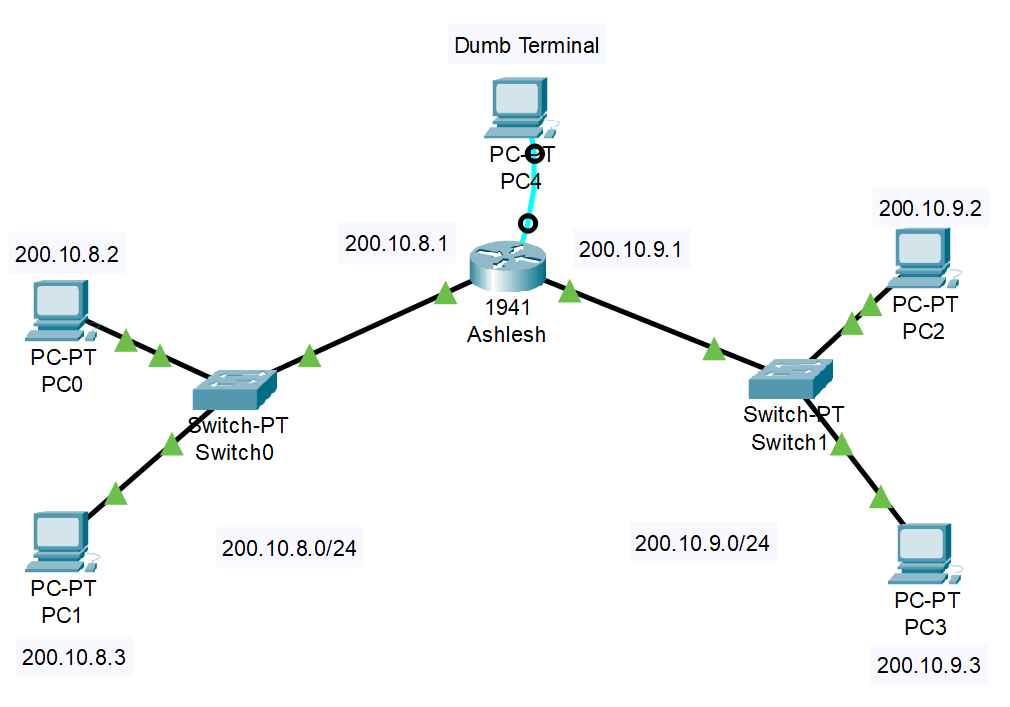
\includegraphics[scale=0.7]{./Figures/simulation.png}
        \caption{Simulated network with two switches and four computers}
        \label{fig:simulation}
    \end{figure}
    The connections as shown in Figure~\ref{fig:simulation} were initially made on Packet Tracer. The router was connected to the switches using two gigabitethernet interfaces. A rollover cable was used to connect the console interface of the router with the RS232 interface of the PC4. Each of the two switches were connected with two separate PCs on the fastethernet interfaces. For basic configurations to be set on the router, the communication port on PC4 was configured with following settings,
    \begin{itemize}
        \item 9600 baud
        \item 8 data bits
        \item No parity
        \item 1 stop bit
        \item No flow control
    \end{itemize}
    Using the termial emulation software on PC4, the router was configured for various settings as needed. Firstly, the hostname of the router was set to \textit{Ashlesh} using the appropriate command from the privileged EXEC mode. Passwords for console line, privileged EXEC mode and virtual terminal were set which were later encrypted too. The interface configuration mode was used to configure the two gigabitethernet interfaces on the router with the appropriate ip addresses and subnet masks. The interfaces were turned on and cross checked for status using the \textit{show running-config} command on the privileged EXEC mode. Individual PCs, viz. PC0, PC1, PC2, PC3 were configured with the instructed ip addresses and subnet masks. Connectivity among the network devices was checked using the ping command as instructed and observations were noted. For further investigations, the default gateway for PC0 and PC1 was set to 200.10.8.1 and that of PC2 and PC3 was set to 200.10.9.1 and connectivity was checked once again.\\
    The various commands used for the basic configuration of router along with their syntax and functions are discussed in Problem 2 and the observations for the simulation and connectivity tests are discussed in Problem 3 within the Exercises section.
    \section{Exercises}
    \problem{What is a router? Explain its role in computer networks.}
    A router is a networking device that is used in a network for receiving, analyzing and forwarding packets incoming into the router to another part of the network. Routers are termed as smart networking devices due to the fact that they can analyze the incoming packets and transfer the data over the network. A router uses the hardware and software combinations to route the packets all the way from the source to the destination. A router is more specifically important for combination of networks, meaning that it connects two or more networks having different network addresses. Large and complex networks are segmented into logical segments called subnets by the router based on the Layer 3 addressing system. The divison of larger networks into smaller logical units allows smaller broadcast domains that lead to a better performance of the overall network. A router is also essential for packet filtering purpose. The simplest form of a router configuration is visible in home routers where the local network is connected to the internet via the router. Here the router acts as a gateway to the vast internet and expands the local network.
    \problem{List out the basic configuration commands of router (that you have used in this lab) with
    their syntax and functions.}
    The configuration commands are used in configuration mode. To access the various configuration modes we need to follow the following commands.
    \syntax{modes}{various router modes}
    \subsubsection*{Configure hostname}
    The hostname of the router can be changed from the command line terminal using \textit{hostname} command. Configuring the hostname of a router aids in debugging and maintenance of the network. 
    \syntax{hn}{configuring hostname}
    \subsubsection*{Configure passwords}
    Passwords for various accesses such as the console line login, privileged EXEC mode, virtual terminal can be set for security purposes. The passwords are stored in plain text format and can be revealed by the \textit{show running-config} command. There is an option for encrypted password as well.
    \syntax{pwd}{configuring router passwords}
    \subsubsection*{Configure interface}
    The two interfaces of the router that are connected to the switches must be configured with proper ip addresses and subnet masks. It is achieved by using the \textit{interface} command in the global configuration mode. The \textit{no shutdown} command enables the interface which can be verified from the \textit{show interfaces} command.
    \syntax{in}{configuring interface}
    \problem{Note down the observation of each steps with necessary commands specified in activity D
    mentioned in the lab sheet and comment on it.}
    \cmdop{hostname}{configuring hostname}
    Changing the hostname of the router is essential for debugging and maintenance purposes. The hostname is displayed on every line of the CLI which aids in proper knowledge of multiple routers in a complex network.
    \subsection*{Before setting default gateway}
    \addtocontents{lol}{\protect\subsection*{Before setting default gateway}}
    \cmdop{0-1}{pinging PC1 from PC0}
    Both PC0 and PC1 are in the same subnet, i.e. 200.10.8.0/24, so the ping goes through successfully without the need of a default gateway.
    \cmdop{0-ra}{pinging interface of router in same subnet from PC0}
    Ping from the PC0 to the router interface 200.10.8.1 terminates successfully since they're in the same subnet.
    \cmdop{0-rb}{pinging interface of router in different subnet from PC0}
    Ping from the PC0 to the router interface 200.10.9.1 terminates with a request timed out error where none of the packets go through successfully. This is due to the fact that the ip address 200.10.9.1 isn't recognized by the subnet 200.10.8.0/24. 
    \cmdop{0-2}{pinging PC2 from PC0}
    Since PC0 and PC2 are in different subnets, i.e. 200.10.8.0/24 and 200.10.9.0/24, the ping from PC0 to PC2 fails without a single packet being transfered. 
    \cmdop{0-3}{pinging PC3 from PC0}
    The ping from PC0 to PC3 fails for the same reason as that of ping to PC2. The difference in subnet causes the ping to fail since default gateways aren't set, so the packets aren't passed on to the appropriate destination.
    \cmdop{3-0}{pinging PC0 from PC3}
    Since PC0 is in a different subnet than that of PC3, the ping fails. The packets aren't routed to the destination since the default gateway for the PCs isn't properly set.
    \cmdop{3-1}{pinging PC1 from PC3}
    The ping fails with a request timed out error due to the same reason as mentioned for PC0. The packet can't go through the router since the source and destination PCs are in different subnets.
    \cmdop{3-rb}{pinging interface of router in same subnet from PC3}
    PC3 is in the same subnet as the router interface with ip 200.10.9.1, which is why the ping successfully terminates with no errors.
    \cmdop{3-ra}{pinging interface of router in different subnet from PC3}
    The ip address 200.10.8.1 is unknown to the subnet 200.10.9.0/24 which is why pinging the interface from PC3 fails with a request timed out error.
    \cmdop{3-2}{pinging PC2 from PC3}
    Since PC2 and PC3 are in the same subnet 200.10.9.0/24, the ping goes through successfully and hence we get a no loss result.
    \cmdop{r-0}{pinging PC0 from router}
    \cmdop{r-1}{pinging PC1 from router}
    \cmdop{r-2}{pinging PC2 from router}
    \cmdop{r-3}{pinging PC3 from router}
    The router is connected to all the PCs which is why a ping from its terminal results in a successfully termination. The hostname of the router is also visible in the outputs which might be of use in complex networks with multiple routers.
    \subsection*{After setting default gateway}
    The observations for ping tests between devices as shown in the section above leads us to a common conclusion that, for a properly set subnet, the ping test succeds no matter the default gateway configuration, but for devices or ip addresses on different subnets, the ping test fails without a single packet transfered. This is because the router has no idea of where the packets should go to reach the appropriate destination. This issue is solved by setting default gateways on devices that match the ip adddresses of their router interface. For instance, the default gateway on PC0 and PC1 should be set to 200.10.8.1 and that of PC2 and PC3 should be set to 200.10.9.1 for the ping from either side to go through.
    \\All the ping tests in this section succed since the gateways are properly set for each PC. The ICMP packets are handed over to the default gateway and the router then routes to the required address without any issue. In real life setup, the default gateway for various devices on our home networks are the ip addresses of the home router. The gateway is essentially the connection of a subnet to another subnet.
    \addtocontents{lol}{\protect\subsection*{After setting default gateway}}
    \cmdop{0-1}{pinging PC1 from PC0}
    \cmdop{0-ra}{pinging interface of router in same subnet from PC0}
    \cmdop{0-rbg}{pinging interface of router in different subnet from PC0}
    \cmdop{0-2g}{pinging PC2 from PC0}
    \cmdop{0-3g}{pinging PC3 from PC0}
    \cmdop{3-0g}{pinging PC0 from PC3}
    \cmdop{3-1g}{pinging PC1 from PC3}
    \cmdop{3-rb}{pinging interface of router in same subnet from PC3}
    \cmdop{3-rag}{pinging interface of router in different subnet from PC3}
    \cmdop{3-2}{pinging PC2 from PC3}
    \cmdop{r-0}{pinging PC0 from router}
    \cmdop{r-1}{pinging PC1 from router}
    \cmdop{r-2}{pinging PC2 from router}
    \cmdop{r-3}{pinging PC3 from router}
    \section{Conclusion}
    The use of cisco packet tracer allowed for a simulated network without the use of any physical devices which would've been difficult otherwise. The network configuration that we achieved during the lab experiment allowed us to learn about the router, its basic configurations, components and need within a network. The various commands for the configuration of a router along with their syntax and functions were also dealt with during the experiment. Connection among networks with different network addresses was performed by using basic setups on the router. The need of a proper default gateway was understood while connecting the two subnets. Logical separation of the two subnets allowed easy debugging for when the pings didn't succed. The report contains the different observations noted during the experiment with some necessary comments on the results.
\end{document}